\documentclass[12pt,twoside]{article}
\usepackage[utf8]{inputenc}
\usepackage{blindtext,changepage,caption,subcaption,graphicx,booktabs,pgfplots,multirow,appendix,mathtools,fancyhdr,pst-plot,floatrow,amsmath,cases,apacite,natbib,caption,tikz,rotating,subcaption,lmodern,graphicx,outlines,amsmath,amsfonts,amssymb,subcaption,mwe, hyperref,sectsty, afterpage}
\usepackage[en-US]{datetime2}
\usepackage{./NJpaper} % my styling file

% ------ % Setting style
\hypersetup{
	pdftex,
	pdfauthor={Nurlan Jahangirli and friends},     % author
	colorlinks=true,       % false: boxed links; true: colored links
	linkcolor=red,          % color of internal links
	citecolor=black,        % color of links to bibliography
	urlcolor=blue           % color of external links
}
% ------- % Setting the graphicspath
\graphicspath{{../../}} 

% ------ % Title page
\urldef{\njahangirliWeb}\url{http://development-review.org/}	\urldef{\njahangirliEmail}\url{nurlan.jahangirli@monash.edu}
\newtheorem{proposition}{Proposition}
\title{A paper}
\author{Nurlan Jahangirli\thanks{Monash U \njahangirliEmail} \\ Monash University}
\date{\color{ChadGreen} \large First draft: t-1 \\ This revision: \today \\ COMMENTS WELCOME}
\runningheads{Nurlan Jahangirli}{A Paper}
	
	
	\begin{document}
\maketitle


% -----------------------------------------------
% 	ABSTRACT
% -----------------------------------------------

\begin{abstract}
	 %\noindent  \input{./sections/abstract.tex}
\end{abstract}
\vspace{1cm}
{\small
	\noindent \textit{Keywords}:  \\
	\textit{JEL codes}: 
}
\thispagestyle{empty}
\newpage
\setcounter{page}{1}



% -----------------------------------------------
% 	BODY
% -----------------------------------------------

%\input{./sections/intro.tex}
%\input{./sections/theory.tex}
%\input{./sections/estimation.tex}
%\input{./sections/discussion.tex}

% -----------------------------------------------
% 	REFERENCES
% -----------------------------------------------
	
\bibliographystyle{chicago}
\bibliography{./ProjectA.bib}

\newpage
\clearpage

\begin{center} \Large \textbf{Appendix -- For Online Publication} \end{center}
\appendix
\numberwithin{equation}{section}
\numberwithin{figure}{section}
\numberwithin{table}{section}

%\input{./sections/appendix_theory}
%\input{./sections/appendix_data.tex}
%\input{./sections/appendix_empirics.tex}



\begin{figure}
	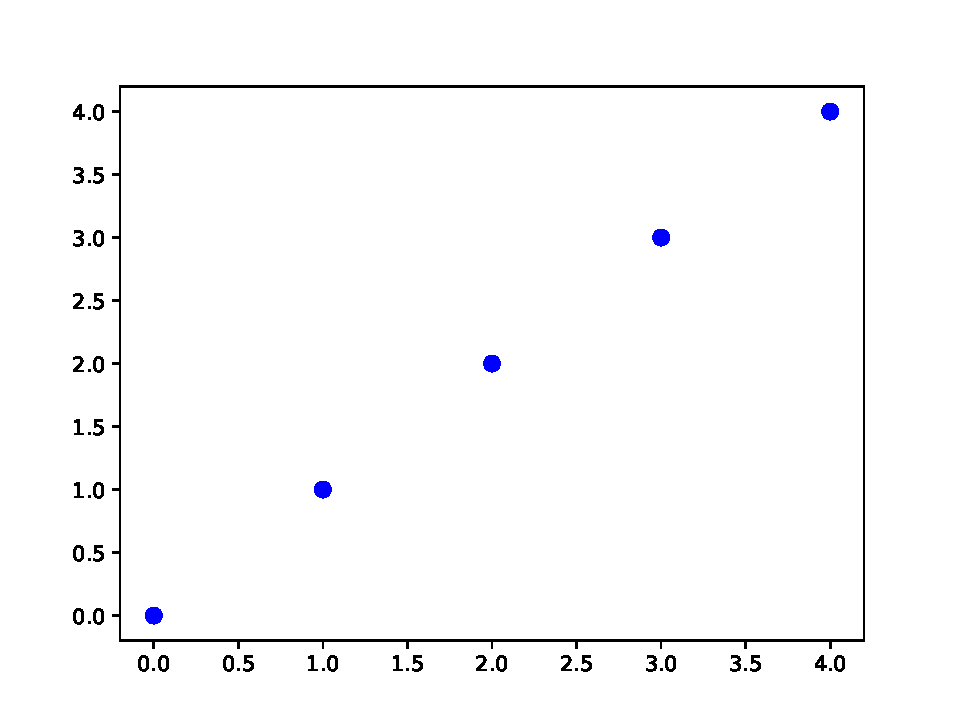
\includegraphics[width=\textwidth]{figures/chart.pdf}
\caption{Example figure. \label{fig:example}}
\end{figure}	



\end{document}

